\begin{frame}{Example: Blacklist}
    Property: no packets from $a$ should reach $d$
    \begin{center}
        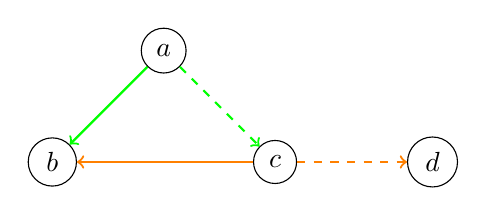
\begin{tikzpicture}[
                node distance={20mm},
                main/.style = {draw, circle},
                s/.style = {->,thick},
                d/.style = {->,thick,dashed} ]
            \node[main] (b) {$b$};
            \node[main] (a) [above right of=b] {$a$};
            \node[main] (c) [below right of=a] {$c$};
            \node[main] (d) [right of=c] {$d$};
            \draw[thick,green,->] (a) -- (b);
            \draw[thick,green,->,dashed] (a) -- (c);
            \draw[thick,orange,->] (c) -- (b);
            \draw[thick,orange,->,dashed] (c) -- (d);
        \end{tikzpicture}
    \end{center}
    \begin{equation*}
        \begin{aligned}[c]
            P   & = p!1                             \\
            Q   & = q!1                             \\
            N   & = F \oplus p?1;N_p \oplus q?1;N_q \\
            N_p & = F_p \oplus q?1;F_{pq}           \\
            N_q & = F_q \oplus p?1;F_{pq}           \\
            F   & = ab \oplus cb                    \\
        \end{aligned}
        \qquad\qquad
        \begin{aligned}[c]
            F_p         & = ac \oplus cb \oplus ab  \\
            F_q         & = ab \oplus cd            \\
            F_{pq}      & = ac \oplus cd \oplus ad  \\
            SDN         & = \delta_{\mathcal{L}} (N
            \parallel P \parallel Q)                \\
            \mathcal{L} & = \s{p!1,p?1,q?1,q?1}     \\
        \end{aligned}
    \end{equation*}
\end{frame}

\begin{frame}{Example: Blacklist}
    Property: no packets from $a$ should reach $d$
    \begin{align*}
        \f{PV} & = \bigvee_{c \in C} c \in \mathcal{F}(ES(\vec v))       \\
        C      & = \s{c \subseteq E | \exists e \in c. l(c) = ad } 
    \end{align*}
    We can define $C(p_1,q_1) = \F$ as an actual cause of $PV$
    using the witness $(C(p_2,q_2),\T,\T)$
    \begin{center}
        \begin{tikzpicture}[scale=0.8]
            \crd{0}{0}{$\emptyset$}
            \crd[left]{-2}{1}{$\s{p_1}$}
            \crd[left]{-2}{2}{$\s{p_1,q_1}$}
            \crd[left]{-2}{3}{$\s{p_1,q_1,ad_1}$}
            \crd[right]{2}{1}{$\s{q_2}$}
            \crd[right]{2}{2}{$\s{p_2,q_2}$}
            \crd[right]{2}{3}{$\s{p_2,q_2,ad_2}$}
            \draw [ultra thick] (-2,1) -- (-2,2);
            \draw [ultra thick] (-2,2) -- (-2,3);
            \draw [ultra thick] (0,0) -- (2,1);
            \draw [ultra thick] (0,0) -- (-2,1);
            \draw [ultra thick] (2,1) -- (2,2);
            \draw [ultra thick] (2,1) -- (2,3);
        \end{tikzpicture}
    \end{center}
\end{frame}